\begin{figure}[th!]
\centering
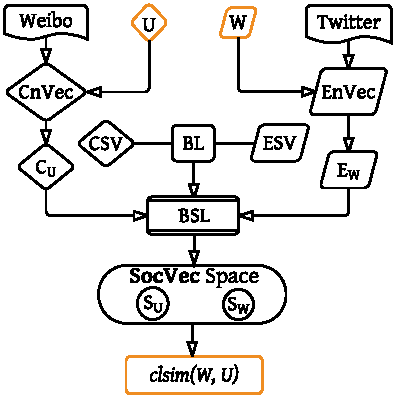
\epsfig{file=figures/overview.pdf, width=0.8\columnwidth}
\caption{Workflow of SocVec for computing the cross-lingual similarity between an English word \textit{W} and a Chinese word \textit{U}. $E_x$, $C_x$ and $S_x$ denote the word vectors of word $x$ in \textit{EnVec} space, \textit{CnVec} space and \textit{SocVec} space respectively.  }
\label{fig:overview}
\end{figure}


\section{Approach}
\label{sec:socvec}

Our problem is that given an English term $W$ and a Chinese term $U$, compute a cross-lingual similarity score, $clsim(W, U)$, that represents the similarity in perception of $W$ and $U$ in the respective cultures. While this paper mainly considers English and Chinese as our target languages, the techniques developed here are language independent and thus can be used for any two natural languages.

 Next sections first discuss  the intuition behind our model informally, then give the overall workflow of our approach, and finally present the details of the~\textit{\socvec}~framework.

%\subsection{Problem Statement}
%Given 
%Imagine we are trying to quantify the cross-lingual similarity between an English word $W$ and a Chinese word $U$, denoted as $clsim(W,U)$, given trained English and Chinese word vectors from microblog corpora (\textit{EnVec}, \textit{CnVec}).
%Although EnVec space and CnVec space may share the same dimensionality, it is unreasonable to directly calculate the similarity between $E_W$(the word vector of $W$ in EnVec) and $C_U$(the word vector of $U$ in CnVec) cross the space, since they are trained separately and the meaning of their dimensions are unmatched.
%\textit{In short, the problem is to devise a reasonable way to calculate the similarity cross heterogeneous word vector spaces and keep the sociolinguistic information in the meantime. }
%
\subsection{The Intuition Behind SocVec}
A very naive solution to the problem is to translate $U$ to its English 
counterpart $U'$ through a bilingual lexicon and then simply consider 
the cosine similarity between $W$ and $U'$ by their word embeddings in English.
However, this solution is infeasible under two situations: 
i) if $U$ is an OOV (Out of Vocabulary) term,
then no $U'$ exists in the bilingual lexicon; 
ii) if $W$ and $U$ refer to the same named entity, $U' = W$, $clsim(W, U)$ remains to be $1$ and cannot capture any cross-cultural difference.

Our intuition is thus to project English and Chinese embeddings to a common third space. This projection needs to carry 
\emph{socio-linguistic} context such as opinions, sentiments and cognition associated with
the terms in respective languages. This information will be encoded as features in
the common space.
%Considering the shortcomings of aforementioned transformation-based solutions, we propose to  
%construct a cross-lingual vector space with respect to sociolinguistic features, instead of transforming a space into another one.
%To construct a universal vector space for multilingual usage, we have to specify the meaning of each dimension for each language.
%Meanwhile, the meaning of the dimensions has to be related to opinion, sentiment, cognition and many other psychological processes to help capture the sociolinguistic information.
%Based on these two requirements, we argue that we should build a Bilingual Sociolinguistic Lexicon and extract word representation using the similarities to each translation pair in BSL as a medium.
%

\subsection{Overall Workflow}
The \textit{\socvec}~model attacks the problem with the help of four external resources: 
i) English Twitter corpus; ii) Chinese Sina Weibo corpus; iii) a bilingual lexicon (denoted as \textit{BL}) between 
 English and Chinese common words; and 
iv) English and Chinese socio-linguistic vocabularies (denoted as \textit{ESV} and \textit{CSV}) consisting of opinion words. 

\figref{fig:overview} shows our framework. First, we train English and 
Chinese word embeddings (known as \textit{EnVec} and \textit{CnVec}) 
from Twitter and Weibo corpus respectively. Then 
we build a bilingual socio-linguistic lexicon (denoted as \textit{BSL}) 
from the bilingual lexicon and
two monolingual socio-linguistic vocabularies. \textit{BSL} is used to map previously incomparable \textit{EnVec} and \textit{CnVec} 
into the common higher-dimensional \textit{\socvec~}space and thus induce two new vectors $S_W$ and $S_U$, 
which are comparable to each other in \textit{\socvec} now. 

\subsection{SocVec Modeling}
\label{sec:model}
In this section, we present the details of building \textit{BSL} and constructing
\textit{\socvec} space.

\subsubsection{Building Bilingual Socio-linguistic Lexicon}
For convenience, we use the term ``social word'' here to represent the words in 
a socio-linguistic vocabulary. The process of building \textit{BSL} is 
illustrated in~\figref{fig:BSL}. 
To build \textit{BSL}, we first use the bilingual lexicon to translate each word 
in \textit{ESV} into several Chinese words. 
Then, we filter out Chinese words that are not in \textit{CSV}. After that, we have a group of Chinese social words as the translations of each English social word. 
The final step of building \textit{BSL} is to construct a 
``pseudo-word'' for each English social word by a pseudo-word generator. 
\begin{figure}[th]
	\centering
	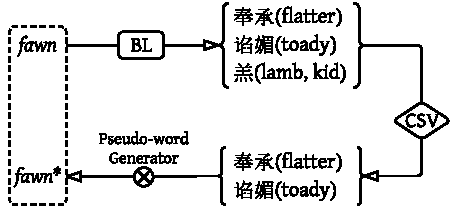
\epsfig{file=figures/BSL.pdf, width=0.85\columnwidth}
	\caption{Generating an entry in BSL for ``\textit{fawn}'' 
		and its pseudo-word ``\textit{fawn}*''.}
	\label{fig:BSL}
\end{figure}

For example, in \figref{fig:BSL}, 
English social word ``\textit{fawn}'' has three Chinese translations in the 
bilingual lexicon, but only two of them are Chinese social words. 
The pseudo-word generator takes the \textit{CnVec} of the two words as 
input and generates the pseudo-word vector of ``\textit{fawn}'', denoted as ``\textit{fawn*}''. 

%A pseudo-word can be either an existing word that is the most representative word 
%in the group of counterparts or a fabricated word whose word vector is 
%the average of all the counterparts.

Denote $\mathbf{C_i}$ as the \textit{CnVec} of the $i^{th}$ out of $N$ Chinese translation words of a given English social word. Four common pseudo-word generator functions are as follows: 
\small
\begin{align*}
	\intertext{ Max.: Maximum of the values in each dimension.}
	Pseudo(\mathbf{C_1},...,\mathbf{C_N}) &= \begin{bmatrix}
	max(C_1^{(1)},...,C_N^{(1)}) \\
	\vdots   \\
	max(C_1^{(N)},...,C_N^{(N)})
	\end{bmatrix}^{\rm T} \\
	\intertext{ Avg.: Average of the values in each dimension.}
	Pseudo(\mathbf{C_1},...,\mathbf{C_N})&=\frac{1}{N}\sum_i^N\mathbf{C_i} \
	\intertext{ W.Avg.: Weighted average value of each dimension with respect to translation confidence (see~\secref{sec:blpre}).} 
	Pseudo(\mathbf{C_1},...,\mathbf{C_N})&=\frac{1}{N}\sum_i^Nw_i \mathbf{C_i} \
	\intertext{ Top: Choose the most confident translation, $\mathbf{C_{top}}$.}
	Pseudo(\mathbf{C_1},...,\mathbf{C_N}) &= \mathbf{C_{top}} \
\end{align*}
\label{sec:pg}
\subsubsection{Projecting EnVec and CnVec into SocVec Space}
Let $B_i$ be $i^{th}$ English word in \textit{BSL},  $B_{i}^*$ be its corresponding Chinese pseudo-word, $\bf{E_x}$, $\bf{C_x}$ and $\bf{S_x}$ be the word vectors of word $x$ in \textit{EnVec}, \textit{CnVec} and \textit{\socvec} respectively and $L$ be the number of entries in the \textit{BSL}. The last step of computing $clsim(W,U)$ is to project $\mathbf{E_W}$ and $\mathbf{C_U}$ to $\mathbf{S_W}$ and $\mathbf{S_U}$ so that they are comparable to each other.
We define the function $f$ to compute cross-lingual similarity between $W$ and $U$ as follows:
\small
\begin{align*}
&clsim(W,U) := f(\mathbf{E_W},\mathbf{C_U}) \\ 
&=sim\left(
\begin{bmatrix}
    cos(\mathbf{E_W},\mathbf{E_{B_1}})\\
    \vdots \\
    cos(\mathbf{E_W},\mathbf{E_{B_L}})
\end{bmatrix}^{\rm T},\begin{bmatrix}
    cos(\mathbf{C_U},\mathbf{C_{B_1^*}})\\
    \vdots \\
    cos(\mathbf{C_U},\mathbf{C_{B_L^*}})
\end{bmatrix}^{\rm T}\right)\\
&=sim(\mathbf{S_W},\mathbf{S_U}) 
\end{align*}
This calculation process is shown in~\algref{alg:alg1}. Here $cos$ stands for cosine similarity, while $sim$ function is a generic similarity
function, for which a number of
metrics can be considered, as we discuss later in \secref{sec:eval}.
\begin{algorithm}[th]
	\DontPrintSemicolon
	\caption{Compute cross-lingual similarity between an English word 
	\textit{W} and a Chinese word \textit{U} } 
    \label{alg:alg1}
	\KwIn{ \textit{EnVec}, \textit{CnVec}, $BSL$ with $L$ word pairs} 
	\KwOut{the cross-lingual similarity $clsim(W,U)$} 
	$E_W$ = word vector of $W$ in \textit{EnVec}\\
	$C_U$ = word vector of $U$ in \textit{CnVec}\\
	$S_W$ =  zero vector with $L$ dimension \\
	$S_U$ =  zero vector with $L$ dimension \\
%	\Comment*[l]{Project $E_W$ into $S_W$}
	\For{$1 \le i \le L$}{
			$B_i$ =  $i^{th}$ English word in \textit{BSL} \\
			$B_i^*$ = Chinese pseudo-word of $B_i$ \\
			$S_W[i]$ = $cos(E_W,E_{B_i})$\\
			$S_U[i]$ = $cos(C_U,C_{B_i^*})$\\
	} 
	\Return $clsim(W,U)$ = $sim(S_W,S_U)$\\
\end{algorithm}

\subsubsection{Parameters Description}
\label{sec:pd}
Here, we briefly summarize the main parameters of \textit{SocVec} model:
\begin{itemize}
\item Two trained monolingual word embeddings, \textit{EnVec} and \textit{CnVec};  
\item A bilingual lexicon;
\item Chinese and English socio-linguistic vocabularies; 
\item Pseudo-word generator function; 
\item Option of similarity function $sim$; 
\end{itemize} 
We conduct several experiments for testing the these parameters in~\secref{sec:mcdne}.
